\section{Introduction}
\label{sec:intro}

 
Engineering is a challenging discipline to study, and doubly so for students from groups that are underrepresented in engineering, who deal with discrimination, bias, microaggressions, and other forms of “othering” during their careers. These groups include racial and ethnic minorities (\eg \cite{Mcgee:2011}), women (\eg \cite{Moss-Racusin:2012}), LGBTQIA+ identifying students (\eg \cite{Cech:2011}) and first-generation college students (\eg \cite{Pascarella:2004,Carrigan, et al., 2019}. These challenges can be compounded when multiple of these identities come into play (\eg \citep{Williams:2014}). Despite significant funding and attention paid to diversity in engineering, the percentage of B.S. degrees awarded to women in 2017 was just 21.3\%.  This is even more distressing because 21.3\% was a 10-year high \citep{Asee 2017}. 

 
Although the experiences of minority populations have been studied for some time now, this is a very challenging problem to make progress on. It can be particularly difficult to effectively measure the impact of problems, and of solutions, on students. This is work that typically must be very specific and focused. For example, take the question of bias against women. It can be difficult to prove that bias exists, and is caused by gender, but in the case of resume assessments, a clever way to measure bias is to vary the name (and nothing else) in a resume. Using this approach, multiple studies have demonstrated bias in assessment of resumes based on presumed gender. In one recent double-blind study, 127 faculty in biology and physics each reviewed an undergraduate resume with a randomly assigned female or male name for a fictional lab manager position \citep{Moss-Racusin:2012}. Men were rated as being more competent, hireable, and worthy of mentoring and higher pay than women. Reviewer gender, seniority, field, and age had no effect on outcome. An earlier psychology study of 238 faculty who received four gender-randomized resumes showed similar outcomes \citep{Steinpreis:1999}. Still, the impact of those biases is hard to measure, especially since they are often small and may take years to add up. However, the impact of small differences in the evaluation of female candidates of 1-5\% (a purported degree to which gender bias affects performance ratings \citep{Barrett:1993}) can be used to simulate how discrimination will impact gender distributions over time in an organization \citep{Martell:1996}, as well as productivity \citep{Cole:1991}. In simulation, such differences accumulate, leading to approximately a 2:1 difference in measures of success between men and women at the most senior levels \citep{Cole:1991,Martell:1996}. 
%More recently, a study in 2014 showed that in an online course, female instructors are given lower student evaluations of teaching than males, if students believe that they're female.  This occurs {\it even if the instructor is actually a male.} This study took place in an introductory course in anthropology/sociology, a field that has a much higher population of female students than engineering \cite{MacNell:2014}.  
%% Here is the ref: L. MacNell, A. Driscoll, and A. N. Hunt.  What's in %%a name: exposing gender bias in student ratings of teaching. %%{\Innovative Higher Education}, 40(4): 291-303, 2014. 

At the end of decades of work, we have a model (though no field test) of impact, and still no solution -- no field-tested technique for reducing this bias, or its impact. And this body of work was focused almost entirely on resume assessment of women, just a small piece of the bigger picture for minority students attempting to succeed in their fields. How, then, can we expect to solve these problems? We argue that what is needed is a far more comprehensive approach to data collection. In the era of big data, a comprehensive change in the way that we collect and assess the college student experience is possible. We can  move from the lab to the field,  connect action to behavior, and  collect longitudinal data. This in turn makes it possible to understand bias in  new ways.  

There is past literature that demonstrates that large-scale longitudinal data collection can help us to understand depression and other mental health factors and how they relate to student outcomes (\eg \cite{wang2014studentlife}). That study depended on occasional survey questions combined with a large amount of passive data collection. By complementing self reports with passive data collection we can use big data to create an image of behavior, while learning about specific challenges that students face through self reports. This ability to connect behavior to experience, in the field, is what past studies lack.  %information about discrimination and bias in the filed that can help us understand it better. 

The technological innovations needed to make this possible are here -- we have access to devices that can passively capture many of the activities that students engage in; and technical approaches that can actively capture the remainder of the information we need to know. This is an exciting era for data collection and analysis and one in which it becomes possible to study issues such as discrimination and bias, at scale and in real-time, and truly understand their impact. This important information will help support the design of effective interventions, policy, and decision making to improve the experiences of not just diverse students in engineering, but all students in engineering. 
 
These insights led us to raise seed money necessary to launch a pilot study with 200 students a year ago. Since then, we have revised our study protocol to further improve it, completed the initial analysis presented in this proposal, and begun year one of data collection with 200 first year students. In both the pilot study and year one, we worked hard to ensure a representative sample of underrepresented groups in engineering (UREs), as shown in Table~\ref{tab:study-participants}. This includes women, underrepresented minorities, first-generation college students, and LGBTQ students. 
While we are still collecting year one data as of this writing, our pilot data shows high compliance and the importance of the rich and varied data that we collect for understanding discrimination: Ninety-one participants from the pilot reported almost 450 separate instances of discrimination and we are able to demonstrate the impact of these experiences on sleep and phone use and connect this to emotional state.  \paula{}
%Our  data show that all of these groups are at risk for discrimination and other obstacles that may impact retention. Further, we argue that an intersectional approach is critical to understanding the challenges these groups face. Thus, we consider discrimination, harassment, and other challenges together with a range of identities in a single holistic study.  

Our proposal is to follow as many of the 200 students from year one as possible for three more years, so that we can truly understand the impact of discrimination on engineering students’ experiences and success. While the data from year one can help to shed light on short term impacts of discrimination, it is only with four years of data that we can learn about important long term impacts such as retention. 

\subsection{Intellectual Merit}
\label{sec:questions}

Our proposed work will leverage the collected data to help improve our theoretical understanding of the impact of discrimination on students; answer important questions about both short and long term impacts of discrimination; shed light on mediating factors such as micro-climates and resilience; and ultimately support intervention design. We  propose to test a model of the student experience (shown in Figure~\ref{fig:model} ) that we believe helps to capture the differential stressors experienced by women and other minorities in engineering in a way that can ultimately be quantified and operationalized. 

As shown in Figure~\ref{fig:model}, and described in more depth in Section~\ref{sec:back}, much is known about the relationship between discrimination and long term stress outcomes such as physical and mental health. (\eg \cite{Ong:2009}). However there are also a number of open questions which will be the focus of our work. These are shown in Figure~\ref{fig:model} in the boxes with dashed lines along the dashed arrows. There are four primary questions that we hope to answer. Here we talk about each and explain why it is important. 

\begin{figure}
    \centering
    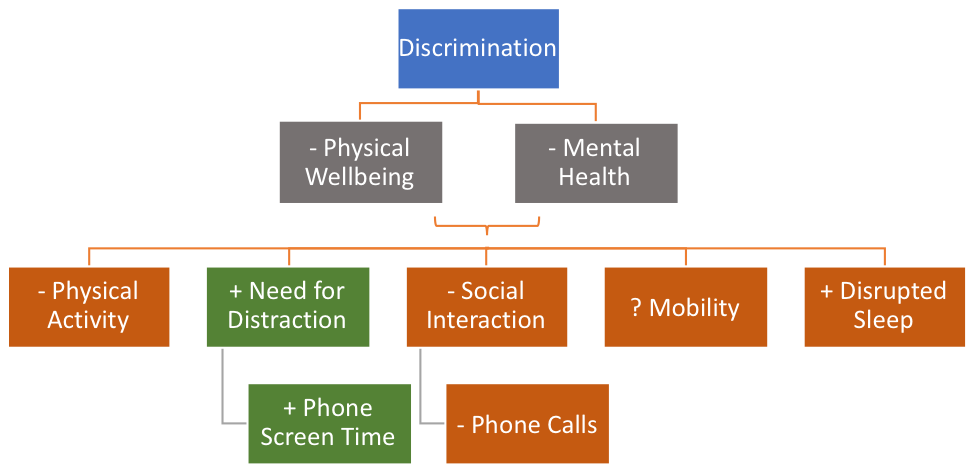
\includegraphics[width=12cm]{img/model.png}
    \caption{Theoretical model relating student experiences to long term outcomes.}
    \label{fig:model}
\end{figure}


\paragraph{Daily Discrimination $\rightarrow$ Short Term Behavior} Our pilot study has already found almost 450 separate instances of  \textit{daily discrimination}, alongside which we have extensive passively collected behavioral data, unlike any former study. Thus, our first research questions ask what we can learn about the impact of daily discrimination from behavioral data. This is particularly important in an educational context where we may find, for example, that discrimination is both more likely at high stress times (such as midterms) and more impactful (if students lose sleep and are thus less well prepared). T
\begin{enumerate}[start=1,label={\bfseries RQ\arabic*}, leftmargin=1cm]
    \item \label{itm:rq-behavior} What is the impact of daily discrimination on short term behaviors? We hypothesize that this is similar to stress, which leads to a second question:
    \item \label{itm:rq-behavior-size} Can we quantify the size of any behavior change due to a daily discrimination event, and the length of time it will last? 
    \item \label{itm:rq-severity-impact} How does the severity of discrimination change these outcomes?
\end{enumerate}

\paragraph{Short Term Behavior $\rightarrow$ Long Term Outcomes} Our second set of questions follow from the first, by extending it to a longitudinal data set. While the impact of discrimination on long term outcomes is something that has been studied, no prior data set has been able to relate short term and long term impacts as ours can. 
\begin{enumerate}[start=4,label={\bfseries RQ\arabic*}, leftmargin=1cm]
    \item \label{itm:rq-short-long} Which long-term outcomes are linked to short-term behavior changes and to what degree?
    \item \label{itm:rq-which-long} Are there specific short term changes that are more likely to relate to long term impacts than others?
    \item \label{itm:rq-severity-long} Are there specific factors such as cumulative severity of discrimination or number of repetitions that predict long term impacts?
\end{enumerate}
 
 \paragraph{Micro-Climates $\rightarrow$ Indirect Impact} Although novel intervention design is out of scope for this proposal, it is our hope that the proposed work will help us to understand the impact of existing micro-climates, which can in turn guide intervention design. We have already identified multiple micro-climates that may impact the discrimination-stress process highlighted in Figure~\ref{fig:model} including STARS, the introductory course sequence the student takes, and participation in SEEEDS mentoring (all are defined in Sidebar~\ref{sidebar:definitions}). We believe that these micro-climates will indirectly impact outcomes through their impact on mediating factors and the likelihood of daily discrimination events. 
 
\begin{WrapText}
\begin{description}[leftmargin=1cm]
\item[STARS] paragraph about STARS
\item[Introductory Sequence] The introductory course experience can have a big impact on the likelihood of discrimination due to the level of competitiveness...
\item[SEEEDS mentoring]
\item[FIGS?]
\end{description}
\end{WrapText}

\begin{enumerate}[start=7,label={\bfseries RQ\arabic*}, leftmargin=1cm]
    \item \label{itm:mc-daily-discrimination} Which micro-climates will reduce exposure to daily discrimination? Which micro-climates will increase exposure?
    \item \label{itm:mc-internal-mediators} Which micro-climates will increase or decrease mediating factors such as resilience and two-way social support? Will this translate into different short-term or long-term behavior outcomes?
    \item \label{itm:mc-external-mediators} Which micro-climates will increase or decrease external mediating factors such as exposure to negative events? Will this translate into different short-term or long-term behavioral outcomes?
\end{enumerate}
 
The contributions of our work will include (1) a more complete theoretical model of the impact of discrimination than previous works
  Our work will also make it possible (2) to document, for the first time, \textit{what behaviors change and in what ways} following acts of discrimination and (3) to demonstrate, for the first time, \textit{which micro-climates reduce that impact} and through what mechanisms. Finally (4) This in turn can guide the development of interventions that help to mediate or reduce the experience of discrimination.
Our goal is to develop a holistic understanding of the impacts of discrimination on the participation and retention of UREs over their college career. 

\subsection{Broader Impact}
\noindent
Our proposed work will improve outcomes for UREs by (1) quantifying impact of unfair treatment (discrimination, harassment and so on)  on students (2) demonstrating to what degree discrimination impacts success and retention of underserved groups (3) quantifying the protective impact of a deployed intervention, an intentionally-created micro-climate targeted at the most at-risk students in Engineering and Computer Science. 

The University of Washington is one of 8 or 10 large flagship public universities in the country. The student experiences in these different settings are likely to be similar in terms of program scale and the range of students and student backgrounds entering the engineering program. This makes it likely that similar interventions will work in similar ways. The impact of discrimination on mental health and physical health is already well-demonstrated in multiple studies. Thus, we expect that our findings will translate to similar large public universities, meaning that we have the potential to impact X 1000 engineers in training each year. We hope that our work will translate to other universities engineering programs working to increase their diversity as well. 

In addition, we will disseminate the results of our proposed work to other universities who are working to retain underserved students in Engineering and Computer Science.  Co-PI Riskin is PI of the UW STARS program, which was founded at UW and Washington State University in 2013,  STARS is an adaptation of the Goldshirt Program at the University of Colorado, Boulder, which is entering its 11th year. Through UW’s leadership, the redshirt model has since been adopted at three additional institutions through a six-institution Redshirt in Engineering Consortium grant from the National Science Foundation (UW, WSU, University of Colorado, Boulder, University of Illinois, Urbana-Champaign, Boise State University, and University of California, San Diego). Through the Redshirt Consortium, UW is engaged in sharing best practices in supporting students from first-generation and low-income backgrounds. 

In the remainder of this proposal, we describe the pilot study that we have already conducted and present some simple preliminary analysis of the data demonstrating promise that our approach can indeed support investigation of these research questions.
 
\subsection{Team}
 
Jennifer Mankoff is the Richard E. Ladner professor in the Paul G. Allen School of Computer Science and Engineering. She has been working with under-represented populations for over a decade (\eg \cite{newman2004perceptions,DBLP:conf/huc/DillahuntMPF09,DBLP:conf/cscw/DillahuntM14,DBLP:conf/huc/DillahuntMP10,DBLP:journals/pacmhci/EarlyHHRWM18,DBLP:conf/chi/OLearyZMR19}). In addition, she has led this study effort at the University of Washington (UW), helped to create the team, and will continue to lead the effort over the remaining years of the study. Her background in Human Computer Interaction has prepared her well to run this effort and her research includes a mix of qualitative behavioral work (\eg \cite{DBLP:conf/huc/DillahuntMPF09,DBLP:conf/chi/MankoffKKRW11}), mixed methods/quantitative behavioral work (\eg \cite{DBLP:conf/ph/CrawfordGSAM14,DBLP:journals/pacmhci/EarlyHHRWM18}), and technical work in behavior modeling (\eg \cite{DBLP:conf/chi/BanovicBCMD16}). 
 
Eve Riskin is Professor of Electrical and Computer Engineering, Associate Dean of Diversity \& Access in the UW College of Engineering, and founder of the UW STARS program.  She is also Faculty Director of UW's ADVANCE program and has been working on diversity and inclusion in engineering for nearly two decades.  She  has published extensively on diversity in engineering education (e.g. EVE-FILL-IN-HERE ).
 
Paula Nurius discrimination
